\chapter{Voorstel nieuwe bewegwijzering}

We zijn bij het bestuderen van de bestaande bewegwijzering in de RAI, AHOY en het VU Ziekenhuis een aantal interessante zaken tegen gekomen. Met als doel het aanpakken van de negatieve punten van de huidige bewegwijzering in de RAI ontwerpen we een nieuw systeem. Indien nodig kijken we hierbij naar de andere twee bestaande systemen.


\section{Eisen}

Uitgaande van de negatieve punten van het huidige systeem in de RAI komen we tot de volgende aanvullende eisen voor een nieuw systeem:

\begin{enumerate}
\item Verschil in verdiepingen moet duidelijker zijn \label{eis:verdiepingen}
\item Indien er plattegronden gebruikt worden moeten deze duidelijke iconen hebben en weinig details bevatten \label{eis:plattegronden}
\item De bewegwijzering moet consistent zijn, dit geldt voor permanente \emph{en} evenement-specifieke bewegwijzering \label{eis:consistentie}
\item Het systeem moet niet afhankelijk zijn van plattegronden \label{eis:afhankelijkheid}
\end{enumerate}

Uiteraard hebben we met meer eisen te maken, bijvoorbeeld eisen waaraan al prima voldaan wordt in de huidige bewegwijzering, of triviale eisen zoals duidelijke betekenis van iconen, juistheid van richting aanwijzers, etc.


\section{Onderdelen}

Ons voorstel voor een nieuwe bewegwijzering bestaat uit de volgende onderdelen:

\begin{itemize}
\item Borden met halnummer bij de ingang van iedere hal
\item Electronische borden bij de ingang van iedere hal waarop de naam van het evenement wordt weergegeven
\item Iconen bij de toiletten, garderobes, liften, EHBO posten, etc.
\item Borden boven de uitgangen van iedere hal met daarop nummers van de hallen waarvoor je de betreffende uitgang gebruikt
\item Iconen boven de uitgangen van iedere hal voor relevante faciliteiten
\item Borden waarop de richting aangegeven wordt naar alle hallen op een aantal strategische punten
\item Iconen met daarbij de richting aangegeven naar faciliteiten op een aantal strategische punten
\item Vereenvoudigde plattegronden op een aantal strategische punten
\item Een groot electronisch overzicht in de aankomsthal van alle evenementen met bijbehorende halnummers
\item Vanen aan het plafond van alle hallen met daarop het halnummer
\end{itemize}

We bespreken deze onderdelen en geven aan wat de voordelen en nadelen zijn ten opzichte van eventuele alternatieven. Ook wordt vermeld aan welke van de door ons gestelde eisen het onderdeel voldoet.


\subsubsection{Borden met halnummer bij de ingang van iedere hal}

Misschien wel het belangrijkste onderdeel van de bewegwijzering. Het moet bij de ingang duidelijk zijn om welke ingang het gaat, anders zal niemand er naar binnen gaan.

We hebben gekozen om halnummers te gebruiken op de permanente borden. Halnamen zijn lastiger te onthouden voor eenmalige bezoekers.

Deze borden helpen de gebruiker te bepalen waar ze zich bevinden en eventueel de locatie van hun doel te bepalen, in het geval ze er dichtbij zijn.


\subsubsection{Electronische borden bij de ingang van iedere hal waarop de naam van het evenement wordt weergegeven}

Naast het halnummer moet bij de ingang van ieder hal ook aangegeven worden welk evenement er plaats vindt. Dit is waar de bezoeker het eerst op af zal gaan.

Omdat de evenementen tijdelijk aanwezig zijn in een hal, gebruiken we hiervoor electronische programmeerbare borden. Het programmeren gebeurt in een centraal systeem, dat voor de juiste weergave op alle electronische borden van ons systeem zorgt.


\subsubsection{Iconen bij de toiletten, garderobes, liften, EHBO posten, etc.}

Hiervoor gelden dezelfde opmerkingen als voor het eerste onderdeel, op de halnummers na. We gebruiken iconen om faciliteiten aan te geven. Dezelfde iconen worden gebruikt in andere onderdelen van ons systeem.


\subsubsection{Borden boven de uitgangen van iedere hal met daarop nummers van de hallen waarvoor je de betreffende uitgang gebruikt}

Om van een hal naar een andere hal te gaan moet je altijd door een uitgang van de hal. Ons voorstel is dan ook om de halnummers die je bereikt door een bepaalde uitgang te gebruiken boven deze uitgang aan te geven, zodat ze vanuit heel de hal te zien zijn. Je kunt dan binnen de hal gemakkelijk zien waar je heen moet lopen voor een bepaalde hal, zelfs al sta je helemaal achterin of in het midden.

Deze borden komen tegemoet aan eis~\ref{eis:afhankelijkheid}, de bewegwijzering mag niet afhankelijk zijn van plattegronden. De route hoeft niet bepaald te worden op een plattegrond, maar wordt (in ieder geval het begin) al aangegeven binnen de hal.


\subsubsection{Iconen boven de uitgangen van iedere hal voor relevante faciliteiten}

Dezelfde redenering als bij het voorgaande onderdeel geldt ook voor het plaatsen van iconen boven de uitgangen van iedere hal. Wanneer je in een hal staat en naar het toilet moet, wil je direct kunnen zien welke uitgang je moet hebben in plaats van eerst naar een muur te moeten lopen om bewegwijzering te vinden.

En ook dit onderdeel helpt de bewegwijzering dus voldoen aan eis~\ref{eis:afhankelijkheid}.


\subsubsection{Borden waarop de richting aangegeven wordt naar alle hallen op een aantal strategische punten}

Het is niet handig en overzichtelijk om overal maar borden te hebben. Beter is om op een aantal strategische punten borden neer te zetten die de richting aangeven naar de hallen. Een strategisch punt zou een plek kunnen zijn waar meerdere hallen hun ingang hebben. Dit onderdeel voldoet aan eis~\ref{eis:afhankelijkheid}.


\subsubsection{Iconen met daarbij de richting aangegeven naar faciliteiten op een aantal strategische punten}

Net als dat je niet overal borden neer zet naar alle hallen, zet je ook niet overal borden neer naar faciliteiten. Ook hier is het verstandig om dit op strategische punten neer te zetten, zodat veel mensen tegelijk er gebruik van kunnen maken en dat toch de overzichtelijkheid gehandhaaft blijft. Dit onderdeel voldoet aan eis~\ref{eis:afhankelijkheid}.

Voor zowel het vorige onderdeel als dit onderdeel geld dat je dit kan vervangen met alleen plattegronden (zoals de RAI dat nu doet). Maar dat heeft als nadeel dat niet veel mensen tegelijk ernaar kunnen kijken. Daarom hebben we ook als eis gesteld dat de bewegwijzering niet afhankelijk is van plattegronden.


\subsubsection{Vereenvoudigde plattegronden op een aantal strategische punten}

Het is voor de bezoeker handig dat er een overzicht is van het hele complex, zodat je gemakkelijker een route kan uitstippelen en beter weet wat er komen gaat. Het is niet zo dat het de primaire bewegwijzering is, maar meer ter ondersteuning. Verder moeten er niet teveel details in zitten. Als de contouren van de hallen worden aangegeven en het verschil in verdiepingen, dan is dat meer dan genoeg. Met een pijl in een afwijkende en duidelijke kleur wordt aangegeven waar je je bevindt op de plattegrond. Dit onderdeel voldoet aan eisen \ref{eis:verdiepingen}, \ref{eis:plattegronden} en \ref{eis:afhankelijkheid}.


\subsubsection{Een groot electronisch overzicht in de aankomsthal van alle evenementen met bijbehorende halnummers}

Door een groot electronische bord in de aankomsthallen kan goed worden weergegeven welke evenementen gehouden worden, en waar ze te vinden zijn. Hierdoor ben je niet afhankelijk van bewegwijzering die georganiseerd wordt door het evenement, en creeer je een consistente omgeving. Daarnaast hebben electronische borden het voordeel dat ze makkelijk gewijzigd kunnen worden en dus makkelijk in onderhoud zijn. Dit onderdeel voldoet aan eis~\ref{eis:consistentie}.


\subsubsection{Vanen aan het plafond van alle hallen met daarop het halnummer}

Het is handig om in de hallen aan het plafond vanen te hangen met het halnummer erop. Zo kan iedereen die op dat moment in de hal aanwezig is zien waar diegene zich bevindt. Je zou het ook op een van de muren kunnen zetten, maar waarschijnlijk is de visibility dan lager. Je moet dan gaan zoeken naar de muur waar het nummer op staat. Dit onderdeel voldoet aan eis~\ref{eis:afhankelijkheid}.


\section{Iconen}

\begin{figure}
\begin{center}
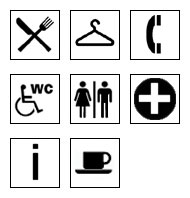
\includegraphics{images/iconen.jpg}
\end{center}
\caption{Overzicht van iconen}
\label{figuur:iconen}
\end{figure}

We gebruiken voor de faciliteiten iconen, zie figuur~\ref{figuur:iconen}. Dit omdat iconen internationaal beter werken dan woorden en minder ruimte innemen. Voor de faciliteiten waar we iconen voor gebruiken bestaan al veel min of meer ``standaard'' representaties. Het is belangrijk dat we deze gebruiken in plaats van andere creatieve oplossingen te bedenken. De bezoekers herkennen de standaard iconen direct en de betekenis is duidelijk.

De gebruikte iconen conflicteren niet met elkaar en zijn ook van een grote afstand goed herkenbaar. Daarnaast passen ze allen in dezelfde stijl.


\section{Electronisch systeem}

Het grote voordeel van electronische borden is dat je gemakkelijk met informatie om kan gaan. Je voert een keer in dat in hal 9 de AutoRAI gehouden wordt, en op alle borden waar dat op weergegeven moet worden kunnen het dan weergeven. Het is dan wel noodzakelijk dat de borden centraal beheerd worden door slimme software.
Een ander voordeel is dat je typefouten kunt verbeteren, of nieuwe namen van evenementen gemakkelijk in kunt voeren. Je hoeft niet een compleet nieuw bordje te maken (maal het aantal plaatsen waar het bordje geplaatst moet worden).

Wanneer dit mogelijk is moet het uiterlijk van de electronische borden zoveel mogelijk aansluiten bij de andere bewegwijzering.
